\procTitle{Напряженные состояния Мельдекского сегмента Ланково-Омолонской разломной зоны}

\procAuthorI{Кондратьев~М.\,Н.}
\procEmailI{mkondratyev85@gmail.com}
\procOrganizationI{СВКНИИ ДВО РАН}
\procCityI{Магадан}

\procAuthorII{Крылов~И.\,А.}
\procEmailII{vagrant99@yandex.ru}
\procOrganizationII{СВГУ, СВКНИИ ДВО РАН}
\procCityII{Магадан}


\makeProcTitleII

\index{k@Кондратьев~М.\,Н.}
\index{k@Крылов~И.\,А.}


Ланково-Омолонская зона является зоной активных разломов право-сдвиговой
кинематики. Разломы отчетливо выражены в рельефе и хорошо выделяются на космоснимках
в~виде протяженной полосы от северного побережья Охотского моря в юго-западной
части зоны, до Чукотского полуострова в северо-восточной части зоны.
Зона ограничивает продолжение активного разлома Улахан на юг и разделяет
Верхояно-Чукотскую и Корякско-Камчатскую складчатые области [3].


Активность Ланково-Омолонской зоны доказана как приуроченностью к ней
дислокаций сейсмогравитационного генезиса [7--9], так и наличием в современном рельефе приразломных правосдвиговых деформаций
с величиной обнаруженных смещений до 2,5\,км [3].

На рис. 1 показано выражение кулис разлома в рельефе в пределах Магаданской области.
На изучаемом участке разломная зона рассекает Туманинский массив
гранитных интрузий позднемелового возраста [2]
и местами пространственно соседствует с серией субпараллельных даек
базальтового состава палеогенового возраста [2] северо-восточного простирания.
В пределах динамического влияния разлома находится, также, Мельдекская
палеосейсмодислокация подтверждающая активность разлома [8].

\begin{figure}[H]
  \begin{center}
    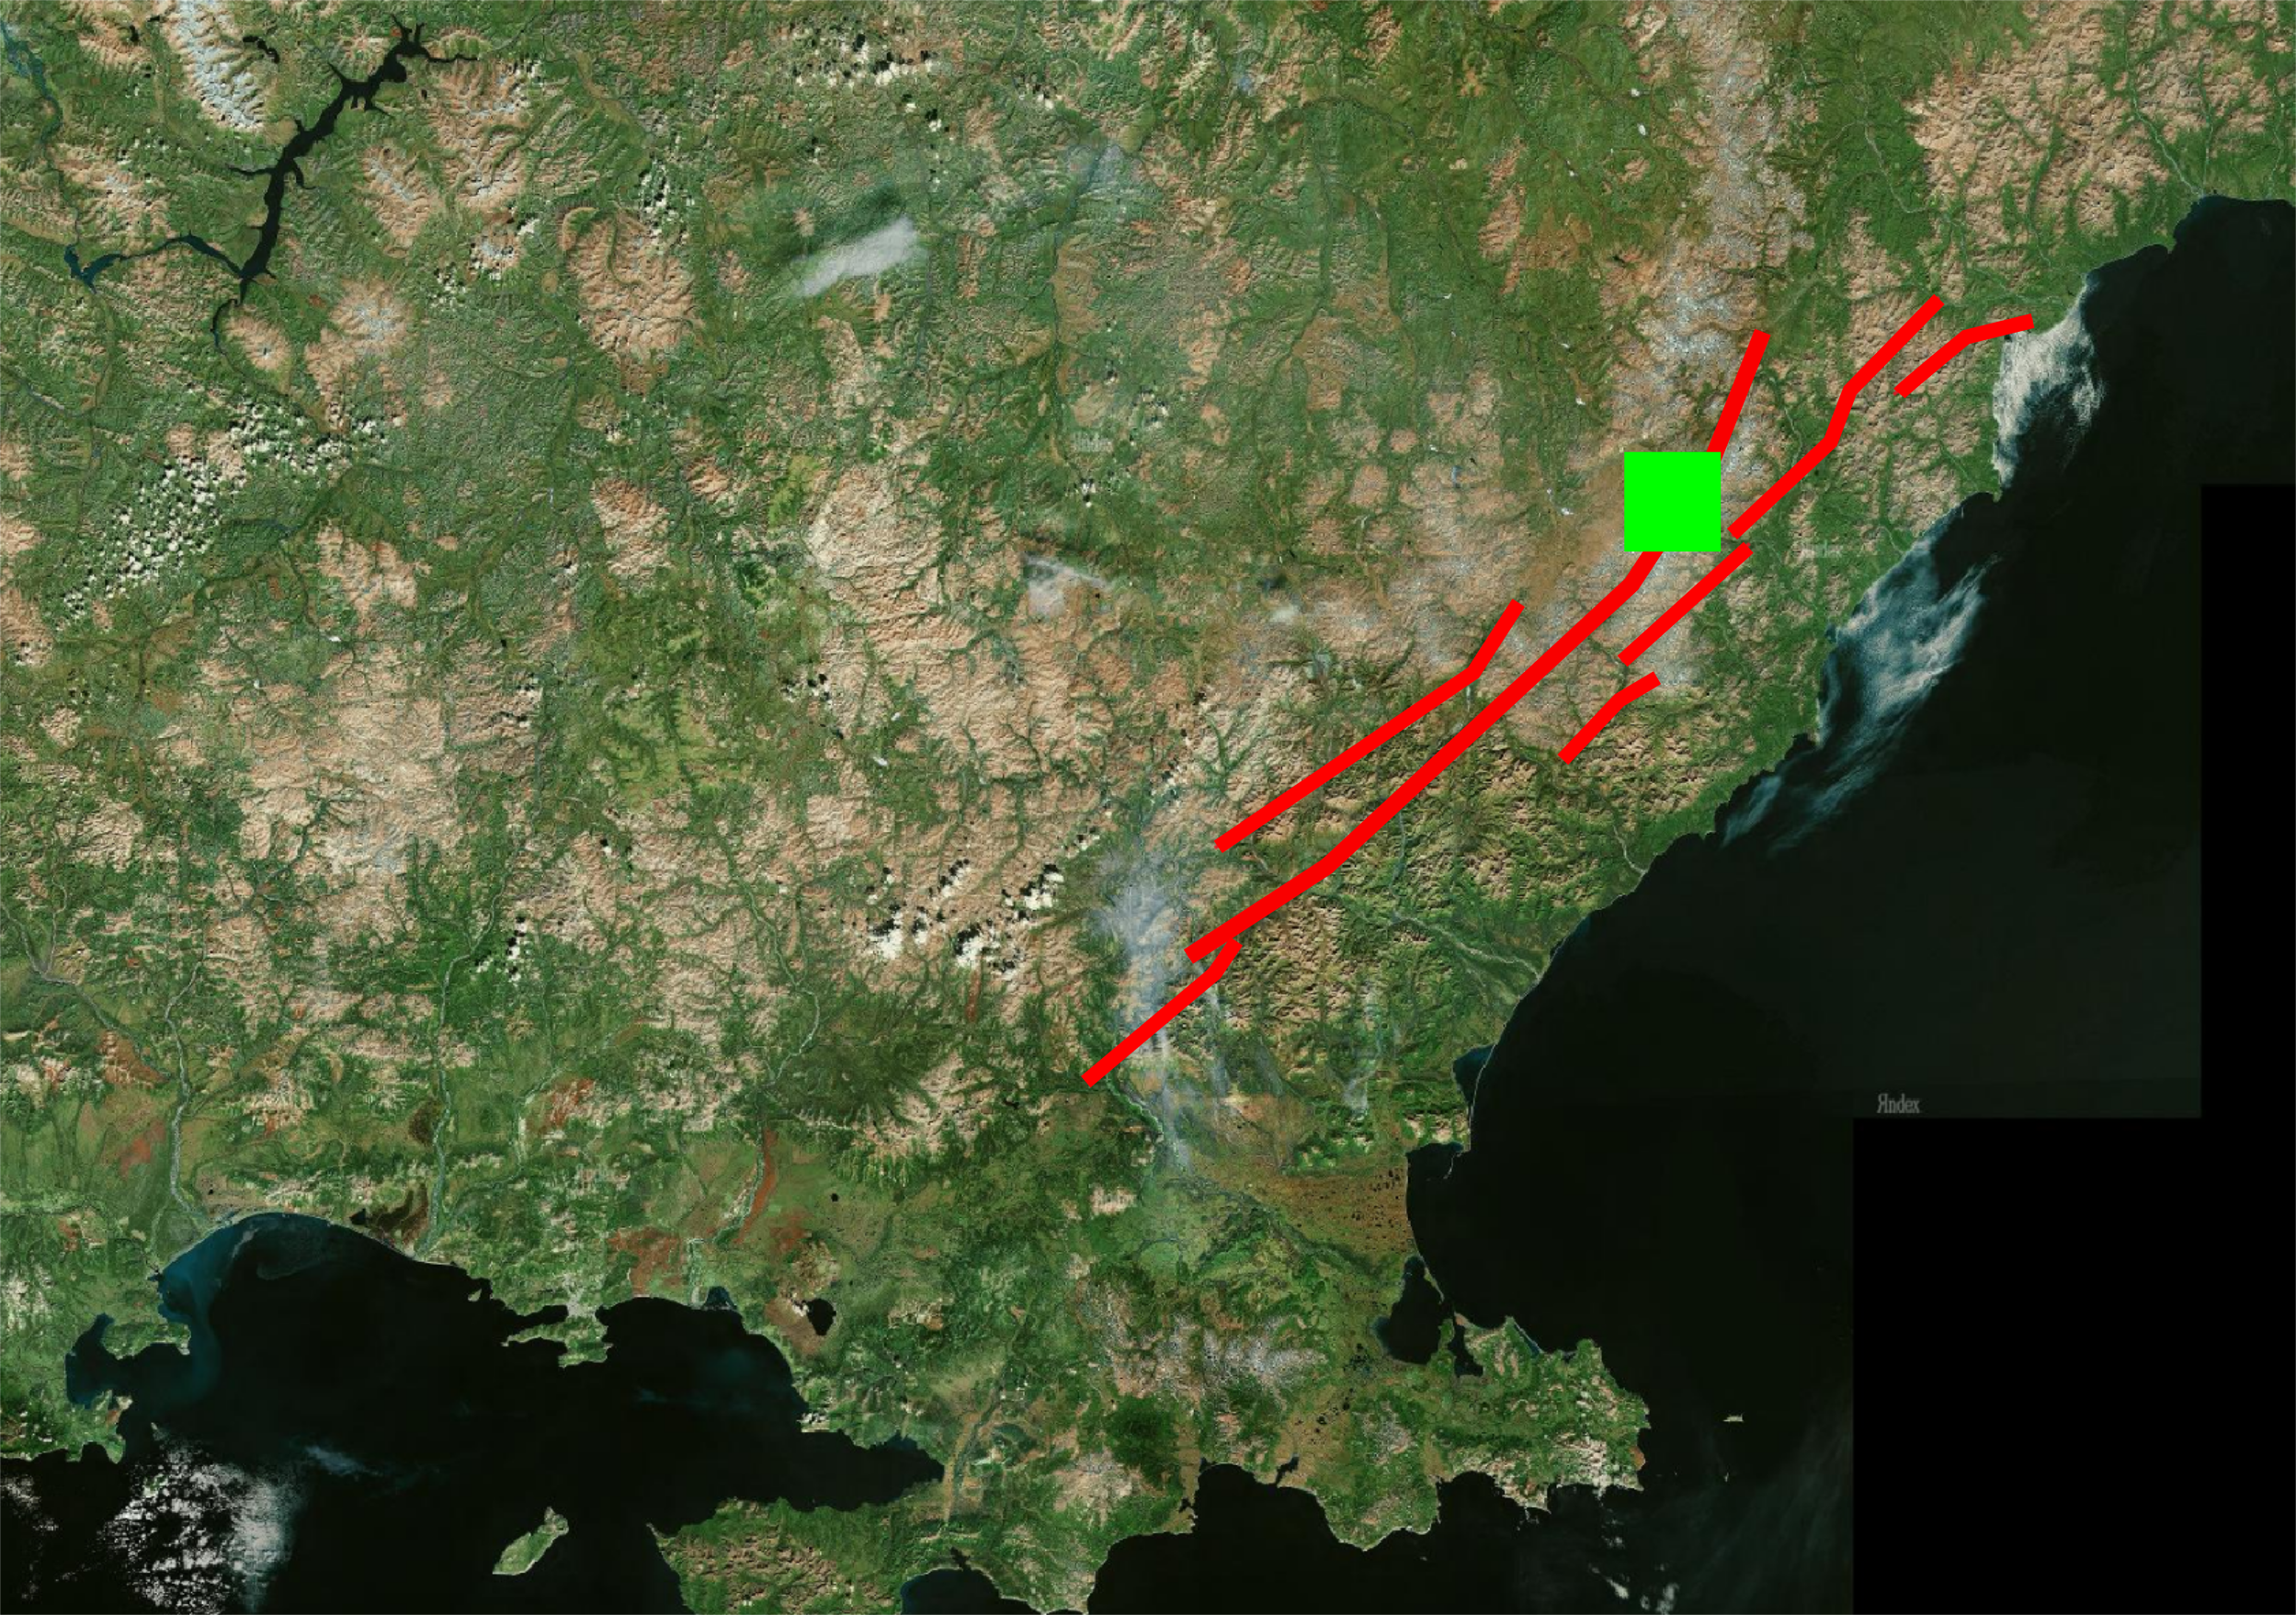
\includegraphics[width=0.7\textwidth]{authors/kondratev-fig1.png}
  \end{center}
  \caption {
	  Выражение Ланково-Омолонской зоны активных разломов в пределах Магаданской области (красные линии). Зеленым квадратом показано положение района работ
}

\end{figure}


С целью восстановления напряженных состояний в зоне действия мельдекского
сегмента Ланково-Омолонской зоны разломов была отобрана серия ориентированных
образцов, произведены массовые замеры тектонической трещиноватости, а также
замеры направления борозд  на зеркалах скольжения.
Результаты анализа собранного материала предоставлены на рис. 2, 3.

\begin{figure}[H]
\begin{changemargin}{0cm}{0cm}
  \begin{center}
    \begin{minipage}[h]{0.6\linewidth}
        \includegraphics[width=1\textwidth]{authors/kondratev-fig2.png}
        \caption{Матрицы плотности тектонической трещиноватости и ориентация осей сжатия и растяжения восстановленные методом Николаева}
        \label{fig:kondratev-fig2}
    \end{minipage}
\hfill
    \begin{minipage}[h]{0.34\linewidth}
      \begin{center}
              \includegraphics[width=0.75\textwidth]{authors/kondratev-fig3.png}
      \end{center}

        \caption{Стереограмма напряженного состояния на основе
    анализа массива зеркал скольжения методом катакластического анализа разрывных смещений Ю.\,Л.\,Ребецкого.
    Нижняя полусфера. Желтым цветом выделен выход на полусферу оси $\upsigma_1$, красным цветом~--- $\upsigma_3$.}
        \label{fig:kondratev-fig3}
    \end{minipage}


  \end{center}
\end{changemargin}

\end{figure}

\clearpage
Напряженные состояния проявленные в изученных обнажениях соответствуют
геодинамическому типу горизонтальный сдвиг, с осью сжатия ориентированной
субширотно, что не противоречит право-сдвиговой кинематике Ланково-Омолонской
зоны разломов. При этом, вид тензора напряжений, определенный методом МКА
соответсвует состоянию сдвигу. Однако, следует отметить, что в пределах
Мельдекской зоны имеется существенная доля взбросовой кинематики что нуждается
в дополнительном изучении.




Основные параметры тензоров напряжений расчитанных на основе выборки из 12 зеркал скольжения замеренных в обнажении находящемся в зоне влияния Ланково-Омолонскогой зоны разломов в раойне оз.\,Мельдек следующие:

\begin{description}[noitemsep]\vspace{-10pt}
\item $\upsigma_1$~--- ориентация вектора растяжения (азимут и угол погружения)~--- 270\dg\,\angl66;
\item $\upsigma_3$~--- ориентация вектора сжатия (азимут и угол погружения)~--- 96\dg\,\angl23;
\item $\upmu_\upsigma$~--- коэффициент Лоде~--- Надаи ~--- 0,12;
\item P~--- редуцированные значения эффективного давления~--- 1;
\item $\uptau$~--- редуцированные значения максимального касательного напряжения~--- 0,2;
\item Тип напряженного состояния~--- горизонтальный сдвиг.
\end{description}



%
\begin{center}
\begin{minipage}[c]{1.0\textwidth}
 \begin{table}[H]
 \begin{center}
 \caption{\bfseries Параметры тензоров напряжений расчитанных на основе выборки из 12 зеркал скольжения замеренных в обнажении находящемся в зоне влияния Ланково-Омолонскогой зоны разломов в раойне оз.\,Мельдек}


 \label{tab:kondratev-tab}
 \medskip\footnotesize

 \begin{tabularx}{1\linewidth}{ c c c c c l}
 \toprule
 $\sigma_1$ &  $\sigma_3$ & $\mu_\sigma$ & $P$ & $\tau$ & Тип напряженного состояния \\
 \midrule

 270\dg\,\angl66  & 96\dg\,\angl23 & \hspace*{0.9em}$0,12$  & $1$  &  $0,2$ & горизонтальный сдвиг \\


 \bottomrule
 \end{tabularx}
 \end{center}

\footnotesize
Примечание:
$\sigma_1$~--- ориентация вектора растяжения (азимут и угол погружения),
$\sigma_3$~--- ориентация вектора сжатия (азимут и угол погружения),
$\mu_\sigma$~--- коэффициент Лоде~--- Надаи,
$P$~--- редуцированные значения эффективного давления,
$\tau$~--- редуцированные значения максимального касательного напряжения.


 \end{table}
\end{minipage}
\end{center}



\begin{thebibliography}{99}
%1
\bibitem{}\BibAuthor{Бачманов~Д.~М., Зеленин~Е.~А., Кожурин~А.~И., Трифонов~В.~Г.} Использование базы данных активных разломов Евразии при решении тектонических задач // Геодинамика и тектонофизика.~--- 2019.~--- №~10\,(4).~--- С.~971--993.~--- DOI:~10.5800/GT-2019-10-4-0453.

\bibitem{}Государственная карта СССР масштаба 1:200 000, серия Магаданская, лист P-56-XXX. / Авт.~А.~Д.~Силинский, ред. В.~Т.~Матвеенко.~--- Магадан, 1969.

\bibitem{}\BibAuthor{Кожурин~А.~И.} Активная геодинамика северо-западного сектора Тихоокеанского тектонического пояса (по данным изучения активных разломов) : диссертация ... доктора геолого-минералогических наук : 25.00.03 / Кожурин Андрей Иванович; [Место защиты: Объединенный институт физики земли РАН].~--- М., 2013.~--- 131~с.

\bibitem{}\BibAuthor{Николаев П. Н.} Методика статистического анализа трещин и реконструкция полей напряжений // Изв. вузов. Геология и разведка.~--- 1977.~--- №~12.~--- С.~103--115.

\bibitem{}\BibAuthor{Ребецкий~Ю.~Л.} Реконструкция тектонических напряжений и сейсмотектонических деформаций: методические основы, поле современных анпряжений Юго-Восточной Азии Океании // Докл. РАН.~--- 1997.~--- Т.~354, №~1.~--- P.~101--104.

\bibitem{}\BibAuthor{Ребецкий~Ю.~Л., Сим~Л.~А., Маринин~А.~В.} От зеркал скольжения к тектоническим напряжениям. Методы и алгоритмы / Институт физики Земли им.~О.~Ю.~Шмидта РАН.~--- М.~: Изд-во ГЕОС, 2017.~--- 234~с.

\bibitem{}\BibAuthor{Смирнов~В.~Н.} Ланково-Омолонская неотектоническая зона разломов // Геофизические модели геологических процессов на Северо-Востоке России.~--- Магадан~: СВКНИИ ДВО РАН, 1996.~--- С.~135--147.

\bibitem{}\BibAuthor{Смирнов~B.~H.} Морфотектоника областей горообразования Северо-Востока Азии : Дисс... доктора наук : 25.00.24 / B.~H.~Смирнов ; МГУ.~--- М., 1995.~--- 350~с.

\bibitem{}\BibAuthor{Смирнов~В.~Н., Важенин~Б.~П.} Сейсмогенные формы рельефа в Туманском хребте (Сев. Приохотье) // Количественная сейсмология  и  сейсмостойкое  строительство  на  Дальнем  Востоке.~--- Южно-Сахалинск~: ИМГиГ ДВНЦ АН СССР, 1985.~--- С.~56--57.
\end{thebibliography}
